\label{sec:Results}

We present a proof-of-principle study of our parameter estimation pipeline, employed in a environment which should
resemble the steps taken after the identification of search triggers. To this purpose, a mock data challenge was
constructed to exercise both the low latency gravitational wave searches as well as the parameter estimation follow-up
processes expected to be applied to GW candidates identified by the search \cite{first2years}. This challenge proceeded
in several stages, each desgined to emulate the anticipated workflow in a low latency BNS detection environment. 

Before beginning, data was constructed consistent with the expected  (median) sensitivity for  2015
from \cite{LIGO-Inspiral-Rates,LIGO-2013-WhitePaper-CoordinatedEMObserving}, documents that describe the evolution of
sensitivity of second-generation detectors.   A population of GW signals from binary neutron stars was added into the
data, as described in \cite{first2years} and reviewed here.   Events in this set (the 2015 MDC data) were distributed
isotropically on the sky, and in uniformly in volume out to \textbf{219} \unit{Mpc}. The BNS injections had uniform
random component masses in $1.2 M_\odot-1.6 M_\odot$ and randomly oriented spins with the dimensionless magnitude not
exceeding 0.05. 
These  (precessing) binary signals  were generated via precessing
SpinTaylorT4 templates at 3.5 PN order \cite{BCV:PTF}, including all known post-Newtonian modes \cite{gw-astro-mergers-approximations-SpinningPNHigherHarmonics}.  


First, the \gstlal{} BNS search was performed over the MDC set, identifying events for further follow up.  We present
parameter estimation results from 450 events seleted randomly from a set of recovered events with false alarm rate
smaller than one per century. This threshold is motivated by the selection criteria outlined
in \cite{LIGO-2013-WhitePaper-CoordinatedEMObserving}. From the reported  search pipeline results, we use the $\mc$ and
$\eta$ coordinates from which the intrinsic search space is extrapolated, a the window for time marginalization (see
Section \ref{sec:time_marg}) is formed around the reported coalescence time $t_r$.  The search pipeline also provides reference power spectral densities $S_n(f)$ utilized in evaluating the likelihood.

In addition to the information provided by the search pipeline, we also make use of the posterior probability of $\alpha$ and $\delta$, provided by \BS. It is expected that such information will be available within a few minutes of trigger identification. The gains in time to convergence in the MC integral are expected to outweigh the loss of time waiting for \BS{} to finish processing if the \BS{} posterior is used as a sampling function for the sky location.

%
% POINT: What code was used
Unless otherwise stated, the likelihoods were evaluated using nonspinning TaylorT4 templates at 3.5 post-Newtonian
order, including only the $(2,\pm 2)$ and $(2,0)$ modes.    As we will discuss at length below, this signal model does \emph{not} include all degrees of
freedom permitted to the binary in the data.  
When evaluating the likelihood,   waveforms started at $f_{\rm low}=40\unit{Hz}$.  The inner product (equation \ref{eq:InnerProduct}) integration uses an inverse power spectrum filter targeting the frequency range $[f_{\rm min},f_{\rm max}]=[f_{\rm min}, 2000\unit{Hz}]$, constructed from the measured power spectrum as described in Appendix \ref{ap:DiscreteData}.  

For each event identified by the GW search pipeline, we distributed the intrinsic points according to the procedure described in Section \ref{sec:itr_placement} and evaluated the Monte Carlo integral $10$ times for each mass point. We outline the form of the priors and sampling functions for each parameter in Table \ref{tbl:priors}.

\begin{table}
\begin{tabular}{r|c}
\hline \\
parameter & physical prior \\
\hline \\
distance ($D$) & uniform in volume \\
inclination ($\iota$) & uniform in $cos\iota$, $\iota$ between $(-1, 1)$ \\
polarization ($\psi$) & uniform in $(0, 2\pi)$ \\
orbital phase ($\phi$) & uniform in $(0, 2\pi)$ \\
declination ($\delta$) & uniform in $\cos\delta$, $\delta$ between $(-\pi, \pi)$ \\
right ascension ($\phi$) & uniform in $(0, 2\pi)$ \\
\hline
\end{tabular}
\caption{\label{tbl:priors}Prior distributions used for the extrinsic parameters in the 2015 MDC study.}
\end{table}

Only distance used an adaptive sampling function, starting initially with a constant function. Our distance prior was uniform in volume out to $d=300\unit{Mpc}$. The declination and right ascension were sampled from the posterior provided by \BS. As used here, the skymap had \textbf{$12\times 64^2$ pixels, roughly one per square degree.}


%\subsection{Advanced Detector Mock Data Challenge}
%\label{sec:BNS_2015_MDC}

%The evolution of the sensitivity of the second generation detectors has been described in \cite{LIGO-Inspiral-Rates,LIGO-2013-WhitePaper-CoordinatedEMObserving}. A mock data challenge using data which posseses a sensitivity which matches the median curve in 2015 from that document was used to test our pipeline. In addition to this data set, a population of GW signals from binary neutron stars was added into the data. The population parameters are outlined here, as well as in \cite{first2years}.

%The \gstlal{} pipeline was used to select events for further study. We present parameter estimation results from 450 events seleted randomly from a set of recovered events with false alarm rate smaller than one per century. This threshold is motivated by the selection criteria outlined in \cite{LIGO-2013-WhitePaper-CoordinatedEMObserving}.


\subsection{Detailed investigation of one event}
%% WHAT FIGURES CURRENTLY ARE : 
%     - https://ldas-jobs.phys.uwm.edu/~evano/skymap_reruns/coinc_id_833/ 
%     : v2 = bayestar as prior and sampler, adapt in distance
%    
%% m1 = 1.21992194653 (Msun)
%% m2 = 1.20069205761 (Msun)
%% s1x = 0.00190996297169
%% s1y = 0.00721042277291
%% s1z = -0.00683548022062
%% s2x = -0.00129437400028
%% s2y = -7.87806784501e-05
%% s2z = 0.00192063604482
%% lambda1 = 0.0
%% lambda2 = 0.0
%% inclination = 2.62300610542
%% distance = 112.5338974 (Mpc)
%% reference orbital phase = 4.29952907562
%% time of coalescence = 966822123.762
%% detector is: H1
%% Sky position relative to geocenter is:
%% declination = 0.678935229778 (radians)
%% right ascension = 4.10562181473 (radians)
%% polarization angle = 6.19411420822

Despite providing complete results in less than one hour, our strategy provides extremely well-sampled distributions and
evidence, with small statistical error.   To illustrate its performance, we have selected a single event, whose
parameters are provided in Table \ref{tab:FiducialEvent:Parameters}.   
%



% POINT: Consistency 
The repeated independent evaluations naturally produced by our algorithm provide a simple self-consistency check,
allowing us to quantify convergence empirically.  
Specifically, at each of the 111 mass points automatically targeted for investigation by our algorithm for this event, we
independently evaluated the integral $\LikeRed$ [Figure \ref{fig:FiducialEvent:LikelihoodVersusMchirpEta}] and construct one- and two-dimensional posterior distributions, from
10 independent evaluations [e.g., Figure \ref{fig:FiducialEvent:Triplot:TriggerMasses}].    
%
As illustrated by example in Figure \ref{fig:FiducialEvent:Triplot:TriggerMasses}, these fixed-mass posterior
distributions are smooth; overlap the true parameters \editremark{Need to add injection cross}; and have errors
consistent  with the previously-reported estimate \editremark{prove me}.  
%
Moreover, as illustrated by Figure \ref{fig:FiducialEvent:Cumulatives:Comparison:TriggerMasses}, each of the 10
independent evaluations make posterior predictions that are consistent with one another.   
%
Finally, as illustrated by Figure \ref{fig:FiducialEvent:Integral:ErrorEstimate}, for each mass point the 10 values of $L_{\rm red}$
are consistent with one another to roughly $1\%$.  
%
Keeping in mind our final reported results combine both all mass points and all 10 evaluations at each mass point, we
anticipate relatively little uncertainty due to sampling error in our current configuration.  


\begin{table}
\begin{tabular}{l|ll}
Parameter & True & Search \\ \hline
$m_1 (M_\odot)$ &  1.22 & 1.26 \\
$m_2 (M_\odot)$ &  1.20 & 1.16 \\
$|\chi_1| $ & 0.01  & 0 \\
$|\chi_2| $ & 0.002 & 0 \\
$d (\unit{Mpc}) $ & 112.5 & - \\
$\iota $ & 2.62 & - \\
($\alpha,\delta$) & (4.106,0.6789) &\\ 
$\rho_{\rm search}$ & 10.85 \\
\end{tabular}
\caption{\label{tab:FiducialEvent:Parameters}\textbf{Fiducial event: True and trigger parameters}: The physical parameters of our injected event, compared
  with the parameters provided by the search and used to target our parameter estimation followup.
}
\end{table}

% POINT: Posterior in mc, eta
To construct confidence intervals in $\mc,\eta$, we adopt a uniform prior in $m_1,m_2$ with $m_1,m_2\in[1,30]M_\odot$
and $m_1+m_2\le 30$: inside the specified region, the prior density is $p(m_1,m_2)dm_1dm_2=2 dm_1 dm_2/(28 M_\odot)^2$.
Changing coordinates using the Jacobian $d(m_1,m_2)/d(\mc,\eta)= \delta \mc/M^2 = \delta \eta^{6/5}\mc^{-1}$ where
$\delta = (m_1-m_2)/M = \sqrt{1-4\eta}$, we find the prior density in $\mc,\eta$ coordinates is
\begin{eqnarray}
p(\mc,\eta) d\mc d\eta =  \frac{1}{392 M_\odot^2} \frac{\mc}{\eta^{6/5}\sqrt{1-4\eta}}
\end{eqnarray}
%
In other words, due to a coordinate singularity, the prior in $\eta$ diverges near the equal-mass line.  
%
This coordinate singularity has a disproportionate impact on comparable-mass binary posteriors.


% POINT
The top panel of Figure \ref{fig:FiducialEvent:LikelihoodVersusMchirpEta} shows contours of the reduced likelihood $\LikeRed$ versus
$\mc,\eta$, derived by interpolating between our discrete grid.   As expected, these contours largely agree with the
Fisher matrix used to construct our grid. 
%
For comparison, the bottom panel of Figure \ref{fig:FiducialEvent:LikelihoodVersusMchirpEta} shows the contours of
$p(\mc,\eta)\LikeRed(\mc,\eta)$, including the strong coordinate singularity near the equal-mass line.  
%
Despite the large log-likelihood and the good agreement between the Fisher matrix and likelihood contours, this
coordinate singularity leads to significant differences between a naive 
Fisher-matrix estimate and the posterior distribution.



\begin{figure*}
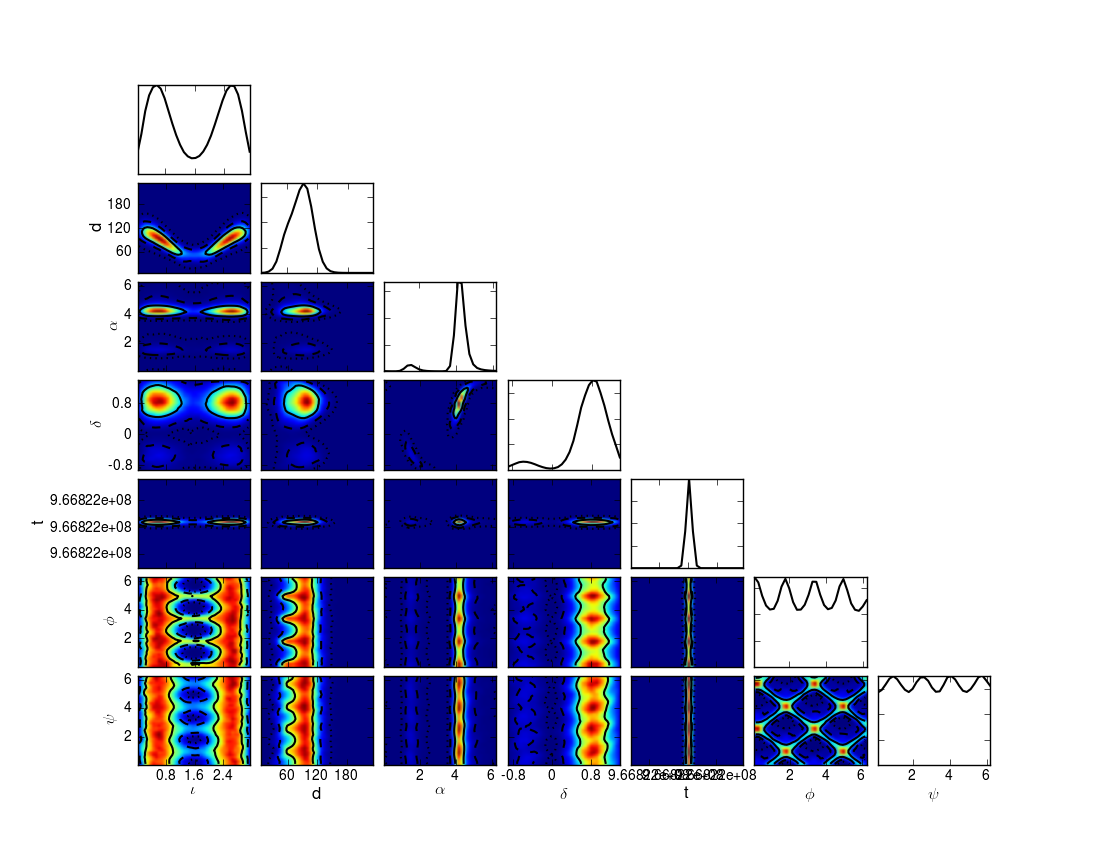
\includegraphics[width=\textwidth]{../Figures/v2runs_coinc_id_833_ILE_triplot_MASS_SET_0}
\caption{\label{fig:FiducialEvent:Triplot:TriggerMasses}\textbf{Posterior distribution in intrinsic parameters, assuming known masses}: For our fiducial event, our predicted
  distribution of extrinsic parameters $d,RA=\alpha,DEC=\delta,\iota,t,\phi,\psi$, for clarity evaluated assuming at the
  mass parameters identified by the search.  Extremely similar distributions are recovered at each mass point. 
\ForInternalReference{  \emph{Suggest: show d-cos iota, skymap, and phi-psi only, not full triplot}}
}
\end{figure*}


\begin{figure}
%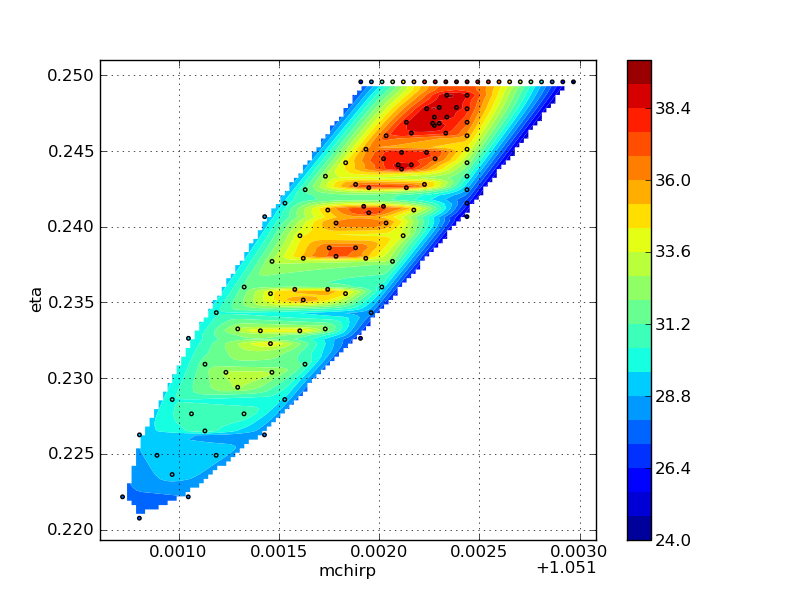
\includegraphics[width=\columnwidth]{../Figures/v2runs_coinc_id_833_mchirp_eta_logevidence}
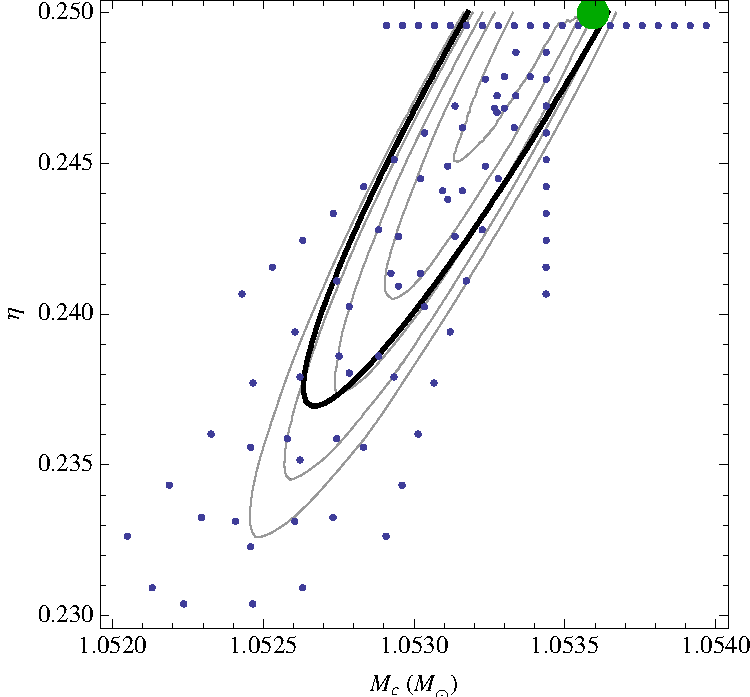
\includegraphics[width=\columnwidth]{../Figures/fig-mma-manual-coinc833-LReducedVersusMcEta}
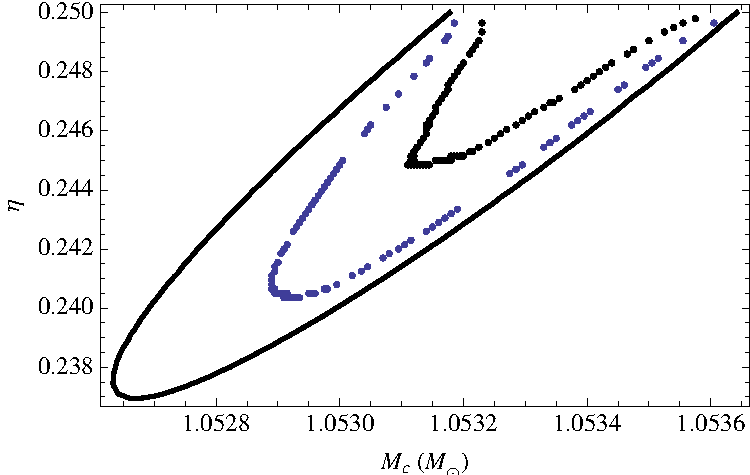
\includegraphics[width=\columnwidth]{../Figures/fig-mma-manual-coinc833-PosteriorMcEta}
\caption{\label{fig:FiducialEvent:LikelihoodVersusMchirpEta}\textbf{Marginalized likelihood and posterior distribution
    versus component masses}: Illustration of intrinsic parameter estimation of a spinning NS-NS event using
    nonspinning templates.  \emph{Top panel}: 
For our fiducial event,
  contours of the log of integrated likelihood $\ln \LikeRed$ versus component masses, represented in $\mc,\eta$
  coordinates.  Points indicate the mass grid adopted; thin contours show isocontours of the (interpolated)
  $\ln \LikeRed=35,36,37,38,39$; and the solid green point shows the injected parametes.   For comparison, the thick black curve corresponds to the 90\% confidence interval
  predicted by combining the network SNR reported by the search ($\rho_{\rm search}$ in Table \ref{tab:FiducialEvent:Parameters}) and the (effective)
  Fisher matrix used when placing test points, as in \cite{gwastro-mergers-HeeSuk-FisherMatrixWithAmplitudeCorrections,gwastro-mergers-HeeSuk-CompareToPE-Aligned,gwastro-mergers-HeeSuk-CompareToPE-Precessing}.  
\emph{Bottom panel}: The 90\% (blue) and 68\% confidence interval (black) derived from the posterior $\LikeRed(\mc,\eta)
p(\mc,\eta)/Z$.  For comparison, this figure also includes the same naive Fisher matrix estimate, shown as a thick black
 line.  
 \editremark{Once OK with Ben Farr, add curves from MCMC TaylorF2}
}
\end{figure}



\begin{figure}
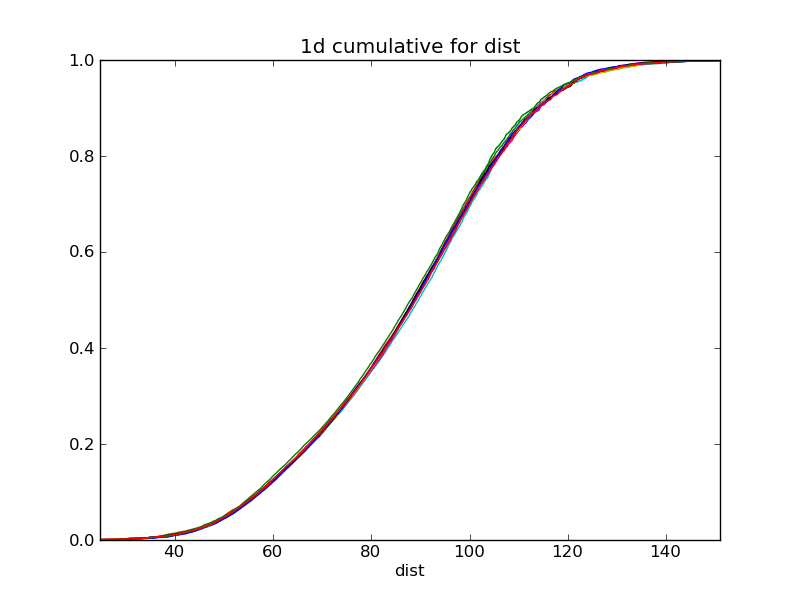
\includegraphics[width=\columnwidth]{../Figures/v2runs_coinc_id_833_cumulative-multiplot-distance-MASS_SET_0}
\caption{\label{fig:FiducialEvent:Cumulatives:Comparison:TriggerMasses}\textbf{Sampling error analysis I: One-dimensional cumulative distribution at fixed mass}:  For each of the 10 independent
  instances used at  the mass  parameters   identified by the search, a plot of the one-dimensional cumulative
  distribution in distance.  These distributions agree to within a few \textbf{(quantify)} percent, qualitatively
  consistent with a naive estimate based on $1/\sqrt{n_{\rm eff}} \simeq 4\%$.   Combining all 10
  independent runs, we expect the final distance posterior has even smaller statistical sampling error
  (\textbf{quantify} $\simeq X/\sqrt{10}$).  Our final posterior
  distributions, having support from several mass points, should have smaller statistical error still.
 \editremark{Once OK with Ben Farr, add curves from MCMC TaylorF2}
}
\end{figure}

\begin{figure}
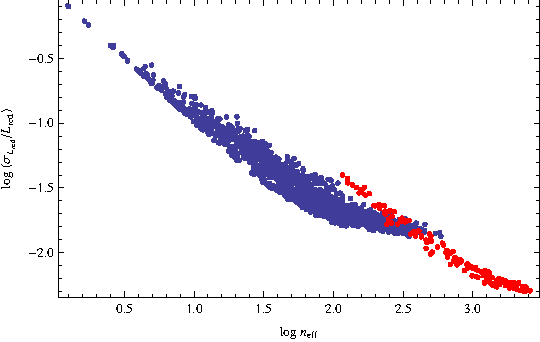
\includegraphics[width=\columnwidth]{../Figures/fig-mma-paper-10202-IntegralErrorVersusNeff}
%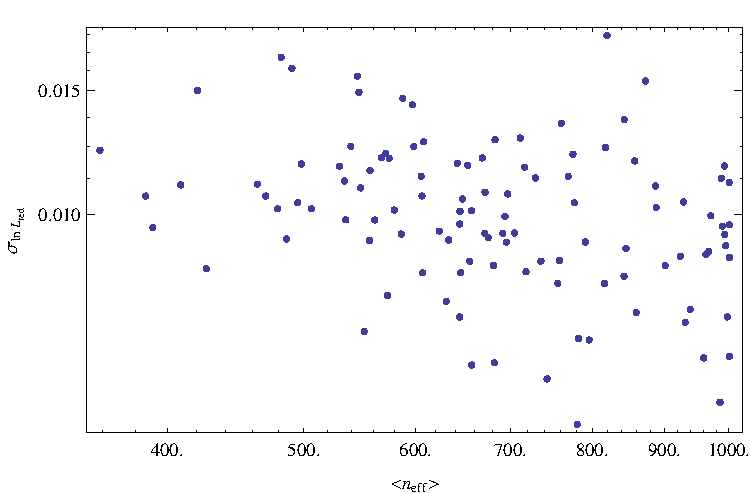
\includegraphics[width=\columnwidth]{../Figures/fig-mma-manual-v2_coinc_833-IntegralVarianceVersusNeff}
\caption{\label{fig:FiducialEvent:Integral:ErrorEstimate}\textbf{Sampling error analysis II: Integral error}: Blue
  points show the standard deviation in $L_{\rm red}$ versus $n_{\rm eff}$ reported for each of the individual code
  instances (1470 trials, corresponding to 147 mass points, 10 times each).  Red points shows the composite error
  $\sigma_{L}$ derived by weighting each of the 10 trials at each mass point, versus the sum of all $n_{\rm eff}$ in
  each trial.   \editremark{Currently showing 10202 - not clear why this iteration is so bad; previous skymap versions had
  sub-percent errors in the composite results? }
%% For each of the 111 mass points evaluated for the fiducial
%%   event, a scatterplot of the mean number of effective samples $n_{\rm eff}$ versus the standard deviation in $\ln
%%   L_{\rm red}$, where at each mass point the mean and standard deviation are calculated over the 10 independent
%%   evaluations performed.  Considering our final prediction for $L_{\rm red}$ combines all 10 events, this figure
%%   suggests $L_{\rm red}$ is known to better than $1\%$ for each mass point.  
% Additionally, this figure illustrates just how many effective samples are available for *each* mass point: thousands.
}
\end{figure}



\subsubsection{Controlled, zero-spin tests}
Though the source investigated here contained two (precessing) spins, our signal model explicitly omitted any spin
effects.  Recent calculations suggest advanced interferometers can weakly constrain astrophysically plausible spins in
binary neutron stars  \cite{2014PhRvL.112j1101F,2014arXiv1404.3180C}. 
%
For this reason, we have carefully repeated our calculations using a  nonspinning source with otherwise identical parameters, inserted into (a) no
noise and (b) the same data used above.   
%
For simplicity, rather than perform a search, we employed the same skymap and coincidence data identified
above.  \editremark{explain triggering issues: time offset needs to be fixed}
%
Results of this comparison are shown in Figure \editremark{XXX}



\begin{figure}
\caption{\textbf{Marginalized likelihood and posterior distribution versus component masses II: Zero spin}:
As Figure \ref{fig:FiducialEvent:LikelihoodVersusMchirpEta}, but for an injection without spin superimposed on (a) identical data
[black] and (b) zero noise [blue]. 
}
\end{figure}



\subsubsection{Validating technical assumptions}



* \editremark{DISCRETE SKY  - resolution limitations? NOT DISCRETE SKY?}

* Validating seperability of posteriors

\subsection{Ensemble of events}

If our estimates for the one-dimensional cumulative distributions $P(<x)$ are unbiased and if $x_*$ is a random variable
consistent with the prior, then $P(x_*)$ should be a uniformly-distributed random variable.   To test this hypothesis,
we use the one-dimensional posteriors provided by the MDC.
%% we perform repeated simulations, where each injected event was drawn from our prior:
%% \begin{itemize}
%% \item 2015 BNS MDC:   We selected \nEventsMDC{} events from the 2015 BNS MDC, identified by the \gstlal{} pipeline.  While all events
%%   have two-dimensional skymaps produced by \BS{}, the analysis presented below did \textbf{not} use two-dimensional skymaps.

%% While the NS-NS binaries in the 2015 MDC had generic spins, our parameter estimation model assumed zero spin.
%% \end{itemize}

% POINT: pp plots for an ensemble of events
For each parameter $x$, each colored curve in Figure  \ref{fig:pp:2015Ensemble} is  the fraction of events with
estimated cumulative probability $P(<x_*)$ at the injected parameter value $x_*$.  
Specifically, if $P(x_{*q})$ are the sorted cumulative probabilities for the $q=1\ldots n$ events with
$P(x_{*1})<P(x_{*2})$, then the points on the plot are $\{P(x_{*,q}),q/n\}$.  
%

\begin{figure}
%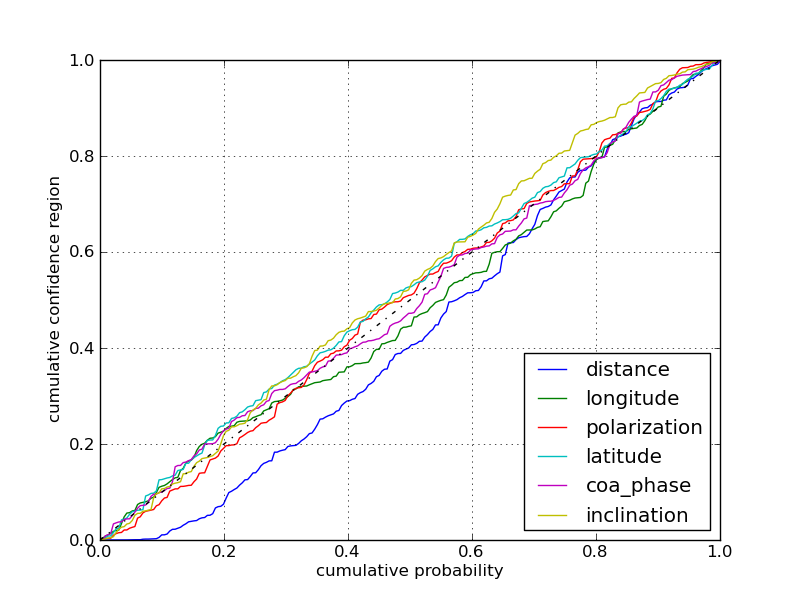
\includegraphics[width=\columnwidth]{../Figures/2015_BNS_MDC_pat_and_chris_pp_plot}   % Original runs
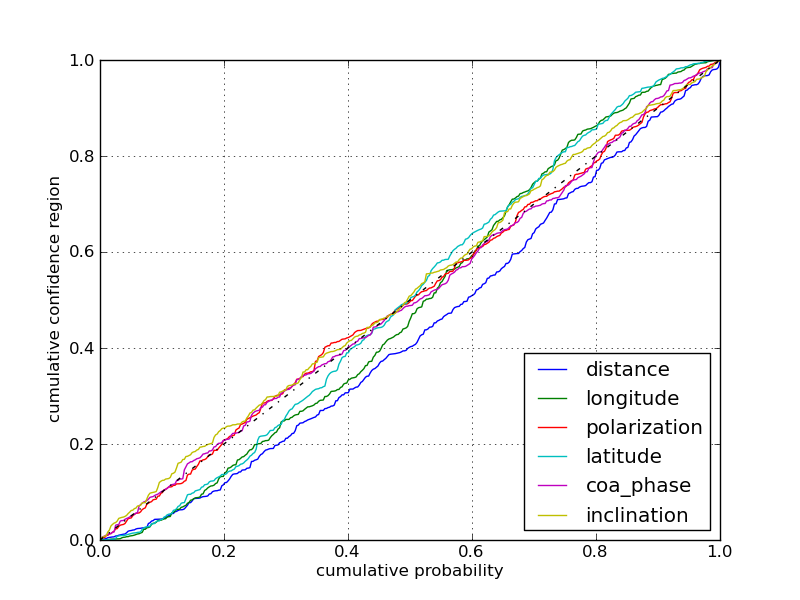
\includegraphics[width=\columnwidth]{../Figures/v1_2015_BNS_MDC_skysampling_pp_plot}  % Bayestar as prior and sampling prior
\caption{\label{fig:pp:2015Ensemble}\textbf{PP plot for ensemble of XXX NS-NS events}: \emph{Top panel}: For \textbf{X} randomly-selected NS-NS binaries, a plot of
  the cumulative distribution of $P_\theta(\theta_k)$ for each extrinsic variable $\theta=d,RA,DEC,\iota,\psi,\phi_{\rm
    orb}$.  \editremark{Beware: currently non-skymap code}
\emph{Bottom panel}: The sky area associated with higher-probability pixels than the true sky position of the source. \textbf{CREATE}
}
\end{figure}

{\color{blue} Integrate: The event selection process outlined \ref{sec:BNS_2015_MDC} introduces a small selection (Malmquist) bias, described in Figure \ref{fig:SearchSelection}, which slightly disfavors edge-on binaries relative to our prior.  Our parameter estimation strategy does not account for selection biases; for a sufficiently large ensemble of events, small deviations between the statistical properties of our posteriors and the ensemble are expected. }

\begin{figure}
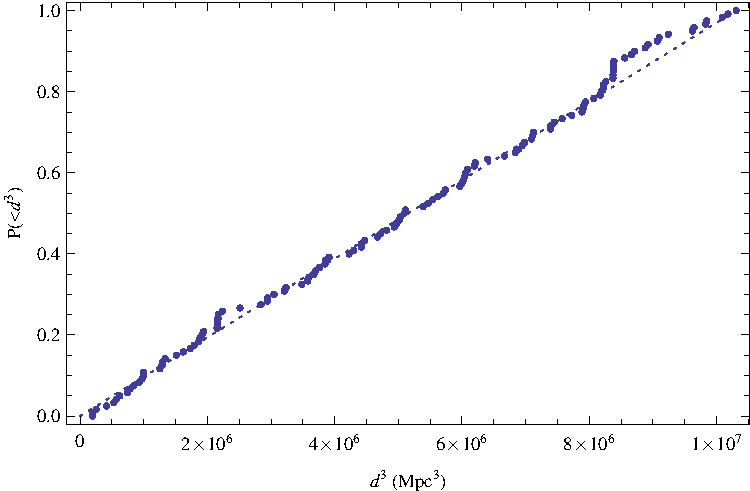
\includegraphics[width=\columnwidth]{../Figures/fig-mma-manual-2015MDC-SelectedEvents-DistanceCumulative}
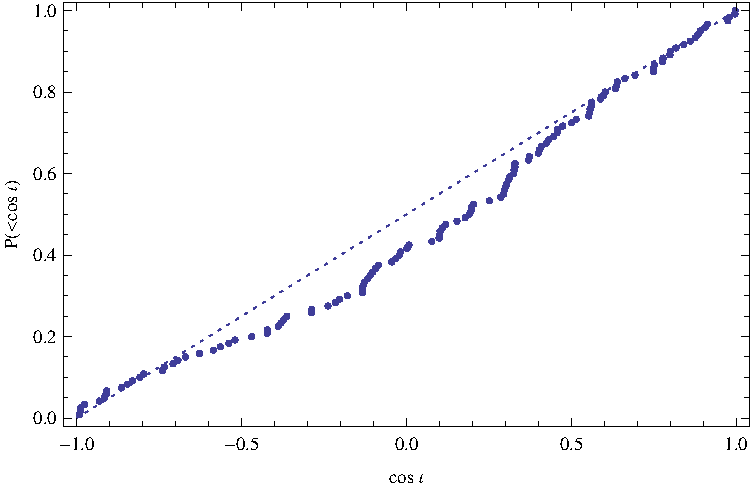
\includegraphics[width=\columnwidth]{../Figures/fig-mma-manual-2015MDC-SelectedEvents-CosIotaCumulative}
\caption{\label{fig:SearchSelection}\textbf{Selection biases}: For the 450 (\textbf{currently 120}) events used in our followup study, the cumulative distribution of $d^3$
  and $\cos \iota$.  In the absence of selection biases and in the limit of many samples, these two parameters should be
  uniformly distributed; small deviations away from uniformity reflect selection biases and sampling error.
}
\end{figure}


\subsection{Scaling}

For a quasicircular compact binary, it is well-known that the time to coalescence from a given GW frequency scales as
$t(f) \propto f^{-8/3}$. As the sensitivity of detectors improves at low frequencies, this requires the use of considerably
longer waveforms for detection and parameter estimation. For example, the initial LIGO detectors were sensitive down
to 40 Hz, while the advanced LIGO detectors could be sensitive down to 10 Hz. To cover extra low frequency
portion would require waveforms that are $\approx 40$ times longer.

Traditional Bayesian parameter estimation is computationally limited by waveform generation and
likelihood evaluations. Both of these are linearly proportional to waveform length. Note that the likelihood evaluations 
involve computing an inner product as in Eq.~\ref{eq:InnerProduct}, 
which is approximated as a finite sum. The number of points in the sum is determined by the length of the waveform 
and data being analyzed, which is why the cost of likelihood evaluations scales with waveform length.
Therefore, one would expect the cost of Bayesian parameter estimation using a seismic cutoff of $f_{\rm min} = 10$ Hz
to be roughly 40 times more expensive than the same analysis using $f_{\rm min} = 40$ Hz.

The method proposed here is not computationally limited by waveform generation. Recall that for each point
in the intrinsic parameter space we compute the waveform and the inner products between the various modes
and the data (the assorted $Q_{k,lm}$, $U_{k,lm,l'm'}$, $V_{k,lm,l'm'}$) only once. We then integrate over the 
extrinsic parameters, which involves evaluating $F_+ + i F_\times$ and the $Y^{(-2)}_{lm}$'s for 
different values of the extrinsic parameters.
While generating the waveform and computing inner products does scale with waveform duration, 
this cost is insignificant (even for $f_{\rm min}=10$ Hz) compared to the integration over extrinsic parameters,
which is wholly independent of waveform duration.
Therefore, the cost of our method increases only a little as $f_{\rm min}$ is decreased, in contrast to the sharp
increase that occurs for waveform-limited techniques such as traditional Bayesian parameter estimation.
See Fig.~\ref{fig:fmin_scaling}.

\ForInternalReference{
* scaling versus number of harmonics used.  (Aside on truncating harmonics with trivial content...not used presently)
}


\ForInternalReference{
\begin{table}
\begin{tabular}{lll}
$f_{\rm low}$ & $t_{\rm wave}$ & $T_{\rm wall}$ \\\hline
10 & & \\
25 & & \\
30 & & \\
\end{tabular}
\caption{\textbf{Runtime versus starting frequency}: Waveform duration $t_{\rm wave}$ and wallclock time $T_{\rm wall}$  needed to evaluate $L_{\rm red}=\int L p d\theta$
  for one set of intrinsic parameters $\lambda$ versus starting frequency $f_{|rm low}$, for a $m_1,m_2=\textbf{XXX}$
  nonspinning black hole binary.  Waveforms were generated using the  \texttt{TaylorT1} and \texttt{EOBNRv2} time-domain
  codes, respectively.  The
  computational cost does not depend significantly on waveform duration for starting frequencies of interest. 
}
\end{table}
}

\begin{figure}
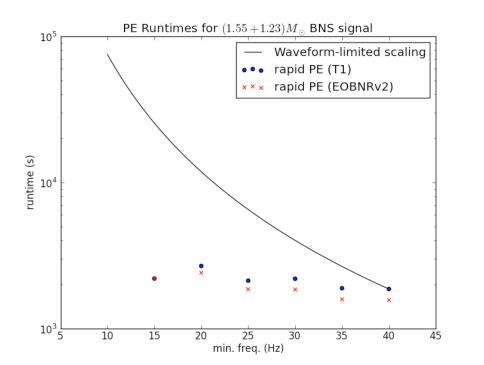
\includegraphics[width=\columnwidth]{../Figures/fig-manual-RuntimeScalingVsFmin.png}
\caption{\label{fig:fmin_scaling}\textbf{Scaling versus frequency}: Points show the runtime of our parameter estimation strategy as a function
  of the minimum frequency $f_{\rm min}$.  For comparison, the solid curve shows the scaling $\propto f_{\rm
    min}^{-8/3}$ expected if our runtime was proportional to the waveform duration (e.g., runtime proportional to the
  number of time samples). 
% INTERNAL REF: coinc_id_17494 was used here.
 Waveforms were generated using the standard \texttt{TaylorT1} time-domain code, with $m_1=1.55 M_\odot$ and $m_2=1.23 M_\odot$. 
}
\end{figure}

